\documentclass[aspectratio=169,11pt]{beamer}

\usetheme{Madrid}
\usecolortheme{default}
\setbeamertemplate{navigation symbols}{}
\setbeamertemplate{footline}[frame number]

\usepackage{amsmath,amssymb}
\usepackage{graphicx}
\usepackage{tikz}
\usetikzlibrary{positioning,calc}
\usetikzlibrary{arrows.meta,decorations.pathmorphing}

\definecolor{RamRed}{RGB}{190,40,45}
\definecolor{RamBlue}{RGB}{30,90,180}
\definecolor{SoftGray}{RGB}{245,245,245}
\definecolor{DarkGray}{RGB}{70,70,70}
\definecolor{MapGreen}{RGB}{48,150,95}
\definecolor{MapGold}{RGB}{235,180,45}

\setbeamercolor{title}{fg=DarkGray}
\setbeamercolor{frametitle}{fg=white,bg=RamBlue}
\setbeamercolor{structure}{fg=RamBlue}

\tikzset{
  v/.style={circle,draw=black,fill=white,inner sep=1.8pt},
  edge/.style={draw=RamBlue,line width=1.25pt},
  topic/.style={draw=black!30,fill=SoftGray,rounded corners=5pt,inner sep=7pt,
    text width=5.8cm,minimum height=1.65cm,align=left},
}

\title[Distance in Graphs]{Distance in Graphs}
\subtitle{Section 1.2 of Harris--Hirst--Mossinghoff}
\author{Jeremy Quastel}
\date{}

\begin{document}

\begin{frame}[plain]
  \centering
  \vspace{0.35cm}
  {\Huge\bfseries Distance in Graphs}\par
  \vspace{0.25cm}
  {\Large Section 1.2}\par
  \vspace{0.15cm}
  {\large Harris--Hirst--Mossinghoff, \emph{Combinatorics and Graph Theory}}\par

  \vspace{0.65cm}
  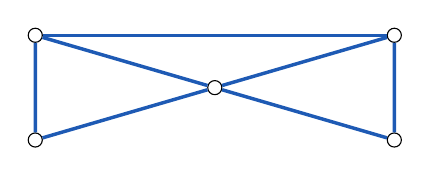
\begin{tikzpicture}[scale=0.95]
    \node[v] (a) at (-2.4,0.7) {};
    \node[v] (b) at (-2.4,-0.7) {};
    \node[v] (c) at (0,0) {};
    \node[v] (d) at (2.4,0.7) {};
    \node[v] (e) at (2.4,-0.7) {};
    \foreach \x/\y in {a/b,a/c,b/c,c/d,c/e,d/e,a/d}
      \draw[edge] (\x)--(\y);
  \end{tikzpicture}

  \vspace{0.3cm}
  {\large Jeremy Quastel}
\end{frame}

\begin{frame}[plain]
\centering
\vspace{0.15cm}
{\Huge\bfseries Today's lecture}\par
\vspace{0.55cm}

\large
\begin{columns}[T,onlytextwidth]
  \begin{column}{0.48\textwidth}
    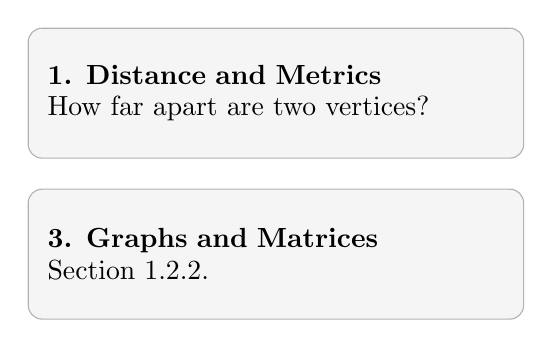
\begin{tikzpicture}
      \node[topic] (a) {\textbf{1. Distance and Metrics}\\[-0.02cm]
      How far apart are two vertices?};
      \node[topic,below=0.38cm of a] (c) {\textbf{3. Graphs and Matrices}\\[-0.02cm]
      Section 1.2.2.};
    \end{tikzpicture}
  \end{column}
  \begin{column}{0.48\textwidth}
    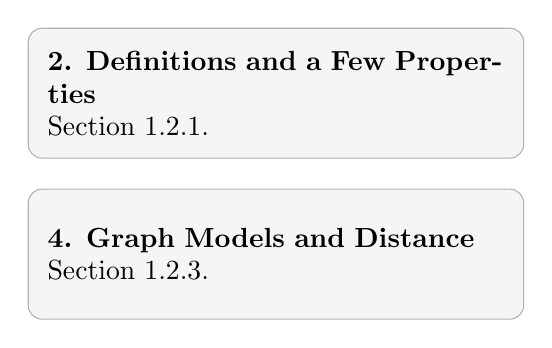
\begin{tikzpicture}
      \node[topic] (b) {\textbf{2. Definitions and a Few Properties}\\[-0.02cm]
      Section 1.2.1.};
      \node[topic,below=0.38cm of b] (d) {\textbf{4. Graph Models and \mbox{Distance}}\\[-0.02cm]
      Section 1.2.3.};
    \end{tikzpicture}
  \end{column}
\end{columns}
\end{frame}


\section{Distance and Metrics}

\begin{frame}{Definition}
\large
\begin{block}{Metric}
Let $X$ be a set. A \textbf{metric} on $X$ is a function
\[
  M\colon X\times X\longrightarrow \mathbb{R}_{\geq 0}
\]
such that:
\begin{enumerate}[i.]
  \setlength{\itemsep}{0.45cm}
  \item $M(x,y)\geq 0$ for all $x,y\in X$, and
        $M(x,y)=0$ if and only if $x=y$;
  \item $M(x,y)=M(y,x)$ for all $x,y\in X$;
  \item $M(x,y)\leq M(x,z)+M(z,y)$ for all $x,y,z\in X$.
\end{enumerate}
\end{block}
\end{frame}


\section{Definitions and a Few Properties}

\begin{frame}{Definition: Graph Distance}
\large
\begin{block}{Graph distance}
Let $G$ be connected. The \textbf{distance} from vertex $u$ to vertex $v$
is the length (number of edges) of a shortest $u$--$v$ path in $G$.

\smallskip
\textbf{Notation:} $d(u,v)$, or $d_G(u,v)$ when specifying the graph.
\end{block}
\vspace{0.10cm}
\begin{center}
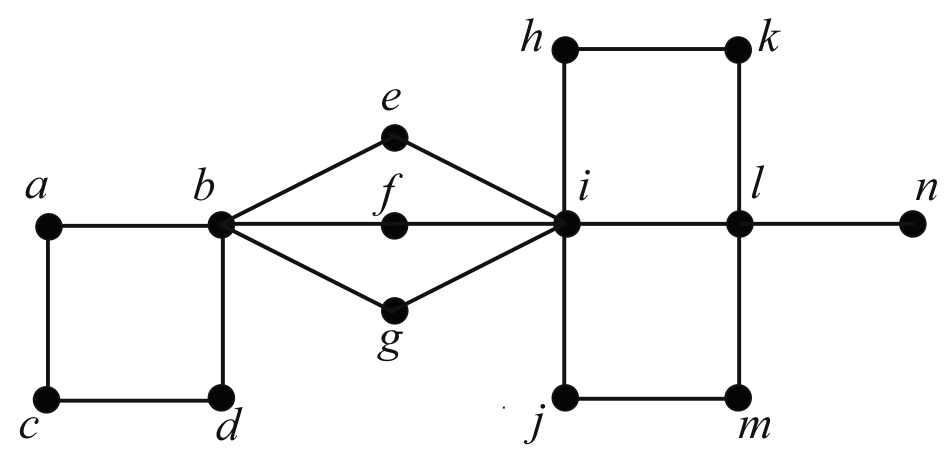
\includegraphics[height=3.15cm]{figure_1_26.png}

\vspace{0.12cm}
In this figure, $d(b,k)=4$. What is $d(c,m)$?
\end{center}
\vfill
{\tiny Source: Harris, Hirst, and Mossinghoff, \emph{Combinatorics and Graph Theory}, 2nd ed., p.~18, Figure 1.26.}
\end{frame}


\begin{frame}{Definition: Eccentricity}
\large
\begin{block}{Eccentricity}
Let $v$ be a vertex of a connected graph $G$. The \textbf{eccentricity} of $v$,
denoted $\operatorname{ecc}(v)$, is defined to be the greatest distance from $v$
to any other vertex. That is,
\[
  \operatorname{ecc}(v)=\max_{x\in V(G)}\{d(v,x)\}.
\]
\end{block}
\vspace{0.05cm}
\begin{center}
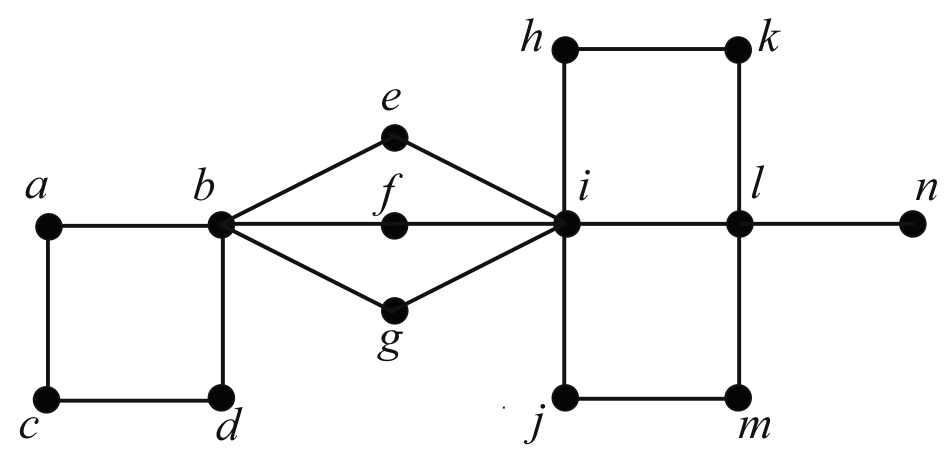
\includegraphics[height=2.35cm]{figure_1_26.png}

\vspace{0.10cm}
What is $\operatorname{ecc}(a)$?\\[0.08cm]
Which vertices have the greatest eccentricity? The least?
\end{center}
\vfill
{\tiny Source: Harris, Hirst, and Mossinghoff, \emph{Combinatorics and Graph Theory}, 2nd ed., p.~18, Figure 1.26.}
\end{frame}


\begin{frame}{More definitions}
\normalsize
\begin{block}{Radius, diameter, center, and periphery}
For a connected graph $G$:
\begin{itemize}
  \setlength{\itemsep}{0.08cm}
  \item The \textbf{radius}, $\operatorname{rad}(G)$, is the smallest vertex eccentricity.
  \item The \textbf{diameter}, $\operatorname{diam}(G)$, is the greatest vertex eccentricity.
  \item The \textbf{center} is the set of vertices $v$ with
        $\operatorname{ecc}(v)=\operatorname{rad}(G)$.
  \item The \textbf{periphery} is the set of vertices $v$ with
        $\operatorname{ecc}(v)=\operatorname{diam}(G)$.
\end{itemize}
\end{block}
\vspace{0.05cm}
\begin{center}
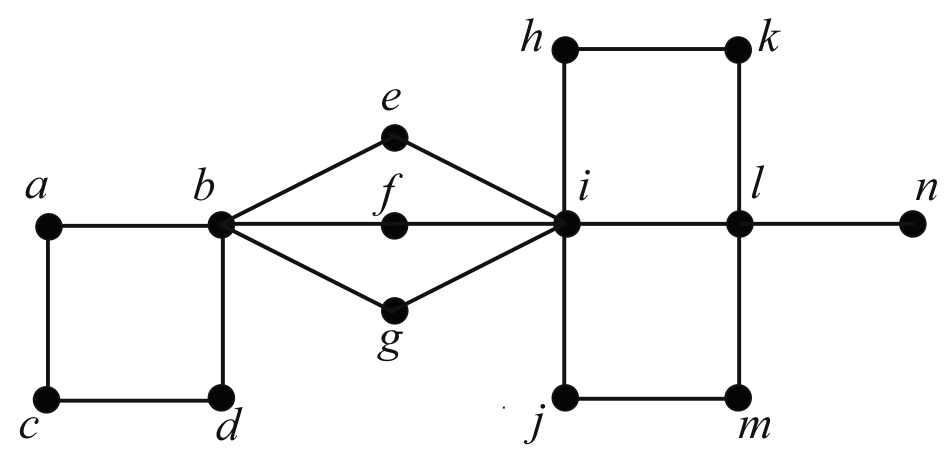
\includegraphics[height=2.25cm]{figure_1_26.png}

\vspace{0.10cm}
\large
What are the radius, diameter, center, and periphery of this graph?
\end{center}
\vfill
{\tiny Source: Harris, Hirst, and Mossinghoff, \emph{Combinatorics and Graph Theory}, 2nd ed., p.~18, Figure 1.26.}
\end{frame}


% Question first, followed by the same slide with the answer revealed.
\begin{frame}[t]{Question}
\large
\vspace{0.25cm}
Is the diameter always bigger than the radius of a graph?
\vfill
\end{frame}

\begin{frame}[t]{Question}
\large
\vspace{0.25cm}
Is the diameter always bigger than the radius of a graph?

\vspace{0.3cm}
\begin{block}{Answer: No}
Equality is possible.
\end{block}

\vspace{0.1cm}
\begin{center}
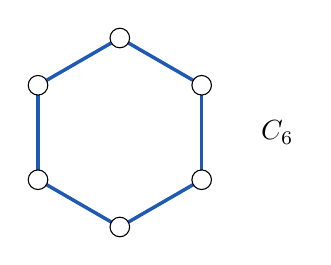
\begin{tikzpicture}
  \foreach \i in {1,...,6}
    \coordinate (p\i) at ({90+60*(\i-1)}:1.2);
  \foreach \i/\j in {1/2,2/3,3/4,4/5,5/6,6/1}
    \draw[edge] (p\i)--(p\j);
  \foreach \i in {1,...,6}
    \node[v,inner sep=2.5pt] at (p\i) {};
  \node at (2.0,0) {$C_6$};
\end{tikzpicture}

\vspace{0.12cm}
On this graph, the diameter and radius are the same:
\[
\operatorname{diam}(C_6)=\operatorname{rad}(C_6)=3.
\]
\end{center}
\end{frame}


\begin{frame}[t]{Theorem}
\large
\vspace{0.15cm}
\begin{block}{Theorem 1.4}
For any connected graph $G$,
\[
  \operatorname{rad}(G)\leq\operatorname{diam}(G)\leq 2\operatorname{rad}(G).
\]
\end{block}
\vfill
\end{frame}

\begin{frame}[t]{Proof of Theorem}
\large
\vspace{0.15cm}
\begin{block}{Theorem 1.4}
For any connected graph $G$,
\[
  \operatorname{rad}(G)\leq\operatorname{diam}(G)\leq 2\operatorname{rad}(G).
\]
\end{block}

\vspace{0.20cm}
\textbf{Proof.}
The first inequality follows directly from the definitions.

\medskip
For the second, choose vertices $u,v$ realizing the diameter:
$d(u,v)=\operatorname{diam}(G)$. Choose a central vertex $c$.
Then
\[
\begin{aligned}
\operatorname{diam}(G)
  &= d(u,v)\\
  &\leq d(u,c)+d(c,v)\\
  &\leq 2\operatorname{ecc}(c)
   = 2\operatorname{rad}(G).
\end{aligned}
\]
\hfill$\square$
\end{frame}


\begin{frame}{Remark}
\large
\begin{block}{Remark}
Graph distance extends to disconnected graphs as follows:
\begin{itemize}
  \setlength{\itemsep}{0.18cm}
  \item Within a connected component, use the usual shortest-path distance.
  \item If two vertices lie in different components, define their distance to be $\infty$.
\end{itemize}
\end{block}

\vspace{0.35cm}
\begin{center}
\begin{tikzpicture}
  \coordinate (a) at (-4,0);
  \coordinate (b) at (-2.5,0);
  \coordinate (c) at (0.3,0);
  \coordinate (d) at (1.8,0.75);
  \coordinate (e) at (3.3,0);
  \foreach \i/\j in {a/b,c/d,d/e}
    \draw[edge] (\i)--(\j);
  \foreach \i in {a,b,c,e}
    \node[v,inner sep=2.5pt,label=below:{$\i$}] at (\i) {};
  \node[v,inner sep=2.5pt,label=above:{$d$}] at (d) {};
\end{tikzpicture}

\vspace{0.35cm}
$d(a,b)=1,\qquad d(c,e)=2,\qquad d(a,c)=\infty.$
\end{center}
\end{frame}


\begin{frame}[t]{Theorem}
\large
\vspace{0.10cm}
\begin{block}{Theorem 1.5}
Every graph is (isomorphic to) the center of some graph.
\end{block}
\vfill
\end{frame}

\begin{frame}[t]{Proof of Theorem}
\large
\vspace{0.10cm}
\begin{block}{Theorem 1.5}
Every graph is (isomorphic to) the center of some graph.
\end{block}

\normalsize
\begin{block}{Proof}
Starting with $G$, form $H$ by adding four new vertices $w,x,y,z$ and the edges
\[
\{wx,yz\}\cup\{xa:a\in V(G)\}\cup\{yb:b\in V(G)\}.
\]
In $H$, $\operatorname{ecc}(w)=\operatorname{ecc}(z)=4$ and
$\operatorname{ecc}(x)=\operatorname{ecc}(y)=3$.

\smallskip
Every $v\in V(G)$ has $\operatorname{ecc}(v)=2$.
Thus the central vertices of $H$ induce precisely $G$.\hfill$\square$
\end{block}
\vspace{0.08cm}
{\centering
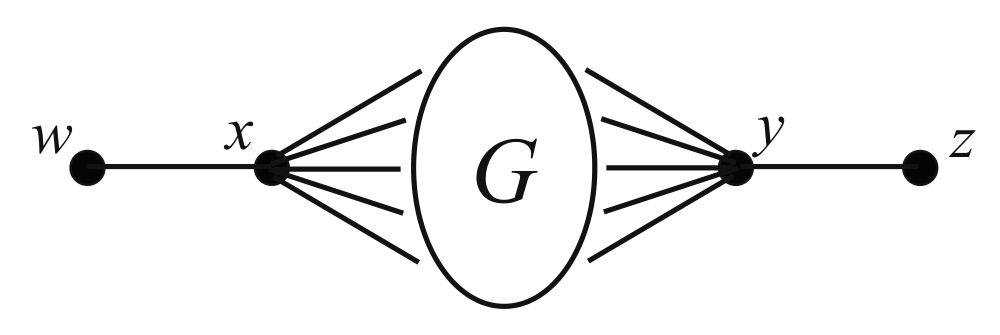
\includegraphics[height=1.2cm]{figure_1_27.png}\par
{\small Figure 1.27. $G$ is the center.}\par
}
\vfill
{\tiny Source: Harris, Hirst, and Mossinghoff, \emph{Combinatorics and Graph Theory}, 2nd ed., p.~19, Theorem 1.5 and Figure 1.27.}
\end{frame}


\begin{frame}[t]{Theorem}
\large
\vspace{0.10cm}
\begin{block}{Theorem 1.6}
A graph $G$ is (isomorphic to) the periphery of some graph if and only if
either all its vertices have eccentricity $1$, or none do.
\end{block}
\vfill
\end{frame}

\begin{frame}[t]{Proof: Forward direction}
\large
\vspace{0.10cm}
\begin{block}{Theorem 1.6}
A graph $G$ is (isomorphic to) the periphery of some graph if and only if
either all its vertices have eccentricity $1$, or none do.
\end{block}

\normalsize
\begin{block}{Proof}
If every vertex of $G$ has eccentricity $1$, then $G$ is complete and is its own periphery.
The one-vertex case is also immediate.

\smallskip
Now suppose no vertex has eccentricity $1$ and $|V(G)|\geq2$.
Form $H$ by adding a new vertex $w$ adjacent to every vertex of $G$.

\smallskip
Each original vertex has a non-neighbor in $G$. In $H$, these vertices are at distance $2$ via $w$, so
\[
\operatorname{ecc}_H(w)=1,\qquad
\operatorname{ecc}_H(v)=2\quad\text{for every }v\in V(G).
\]
Thus the periphery of $H$ is exactly $G$.\hfill$\square$
\end{block}
\end{frame}


\begin{frame}{Forward Direction Diagram}
\normalsize
\begin{block}{Proof: the case with no eccentricity-$1$ vertices}
Suppose $|V(G)|\geq2$ and no vertex of $G$ has eccentricity $1$.
Form $H$ by adding a vertex $w$ adjacent to every vertex of $G$.
Each original vertex has a non-neighbor in $G$, so in $H$ its eccentricity is $2$.
Since $\operatorname{ecc}_H(w)=1$, the periphery of $H$ is exactly $G$.
\end{block}

\vspace{0.12cm}
\begin{center}
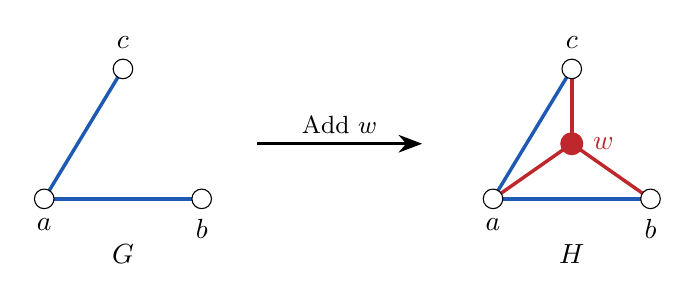
\begin{tikzpicture}
  \begin{scope}[xshift=-3.3cm]
    \coordinate (a) at (-1,-0.65);
    \coordinate (b) at (1,-0.65);
    \coordinate (c) at (0,1.0);
    \draw[edge] (a)--(b);
    \draw[edge] (a)--(c);
    \foreach \i in {a,b}
      \node[v,inner sep=2.5pt,label=below:{$\i$}] at (\i) {};
    \node[v,inner sep=2.5pt,label=above:{$c$}] at (c) {};
    \node at (0,-1.35) {$G$};
  \end{scope}
  \draw[-{Stealth[length=3mm]},line width=1pt] (-1.6,0.05)--(0.5,0.05)
    node[midway,above,font=\small] {Add $w$};
  \begin{scope}[xshift=2.4cm]
    \coordinate (a) at (-1,-0.65);
    \coordinate (b) at (1,-0.65);
    \coordinate (c) at (0,1.0);
    \coordinate (w) at (0,0.05);
    \draw[edge] (a)--(b);
    \draw[edge] (a)--(c);
    \foreach \i in {a,b,c}
      \draw[draw=RamRed,line width=1.25pt] (w)--(\i);
    \foreach \i in {a,b}
      \node[v,inner sep=2.5pt,label=below:{$\i$}] at (\i) {};
    \node[v,inner sep=2.5pt,label=above:{$c$}] at (c) {};
    \node[v,draw=RamRed,fill=RamRed,inner sep=2.8pt,
      label=right:{\textcolor{RamRed}{$w$}}] at (w) {};
    \node at (0,-1.35) {$H$};
  \end{scope}
\end{tikzpicture}

\smallskip
$\operatorname{ecc}_H(w)=\operatorname{ecc}_H(a)=1,\qquad
\operatorname{ecc}_H(b)=\operatorname{ecc}_H(c)=2.$

\smallskip
The periphery is now $\{b,c\}$, not $G$.\\[0.05cm]
{\small Here $\operatorname{ecc}_G(a)=1$, so the hypothesis does not hold.}
\end{center}
\end{frame}

\begin{frame}[t]{Proof: Reverse Direction}
\large
\vspace{0.10cm}
\begin{block}{Theorem 1.6}
A graph $G$ is (isomorphic to) the periphery of some graph if and only if
either all its vertices have eccentricity $1$, or none do.
\end{block}

\normalsize
\begin{block}{Proof}
Suppose $G$ is the periphery of a graph $H$.
Assume, for a contradiction, that $G$ has both a vertex of eccentricity $1$
and a vertex of greater eccentricity.

\medskip
Then $\operatorname{diam}(H)\geq2$.
Choose $v\in V(G)$ with $\operatorname{ecc}_G(v)=1$.
Since $v$ is peripheral in $H$, there is a vertex $w$ such that
\[
  d_H(v,w)=\operatorname{diam}(H)\geq2.
\]
Thus $w$ is also peripheral in $H$, so $w\in V(G)$.
But $v$ is adjacent to every other vertex of $G$, contradicting $d_H(v,w)\geq2$.
\hfill$\square$
\end{block}
\end{frame}


\begin{frame}{Reverse Direction: Diagram}
\normalsize
\begin{block}{Proof}
Suppose $G$ is the periphery of $H$, and $v\in V(G)$ is adjacent to every other vertex of $G$.
As in the proof, choose $w\in V(H)$ with $d_H(v,w)=\operatorname{diam}(H)\geq2$.
Then $\operatorname{ecc}_H(w)=\operatorname{diam}(H)$, so $w$ is also peripheral and must lie in $G$.
Thus $v$ and $w$ are adjacent, contradicting $d_H(v,w)\geq2$.
\end{block}

\vspace{0.15cm}
\begin{center}
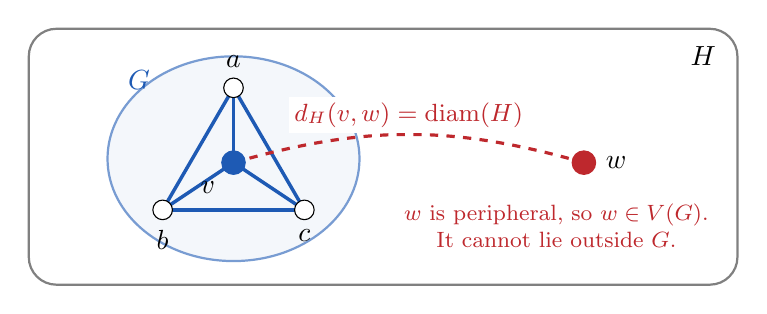
\begin{tikzpicture}
  \draw[rounded corners=10pt,draw=black!50,line width=0.8pt]
    (-4.5,-1.65) rectangle (4.5,1.6);
  \node[anchor=north east] at (4.35,1.5) {$H$};
  \filldraw[fill=RamBlue!5,draw=RamBlue!60,line width=0.8pt]
    (-1.9,-0.05) ellipse (1.6cm and 1.3cm);
  \node[text=RamBlue] at (-3.1,0.95) {$G$};
  \coordinate (a) at (-1.9,0.85);
  \coordinate (b) at (-2.8,-0.7);
  \coordinate (c) at (-1.0,-0.7);
  \coordinate (v) at (-1.9,-0.1);
  \coordinate (w) at (2.55,-0.1);
  \foreach \i/\j in {a/b,b/c,c/a,v/a,v/b,v/c}
    \draw[edge] (\i)--(\j);
  \node[v,inner sep=2.5pt,label=above:{$a$}] at (a) {};
  \node[v,inner sep=2.5pt,label=below:{$b$}] at (b) {};
  \node[v,inner sep=2.5pt,label=below:{$c$}] at (c) {};
  \draw[RamRed,dashed,line width=1.15pt] (v) to[bend left=16]
    node[midway,above,fill=white,inner sep=2pt,font=\small]
      {$d_H(v,w)=\operatorname{diam}(H)$} (w);
  \node[v,fill=RamBlue,draw=RamBlue,inner sep=3pt,
    label=below left:{$v$}] at (v) {};
  \node[v,fill=RamRed,draw=RamRed,inner sep=3pt,
    label=right:{$w$}] at (w) {};
  \node[font=\footnotesize,text=RamRed,align=center] at (2.2,-0.9)
    {$w$ is peripheral, so $w\in V(G)$.\\It cannot lie outside $G$.};
\end{tikzpicture}

\smallskip
The dashed curve represents a shortest path, not an edge.
\end{center}
\end{frame}


\section{Graphs and Matrices}
\begin{frame}{Definition: Adjacency matrix}
\normalsize
\begin{block}{Adjacency matrix}
Let $G$ have vertices $v_1,v_2,\ldots,v_n$ in this order.
Its \textbf{adjacency matrix} is the $n\times n$ matrix $A$ with entries
\[
[A]_{i,j}=\begin{cases}
1 & \text{if $v_i$ and $v_j$ are adjacent,}\\
0 & \text{otherwise.}
\end{cases}
\]
\end{block}
\vspace{0.10cm}
\begin{columns}[c,onlytextwidth]
\begin{column}{0.43\textwidth}
\centering
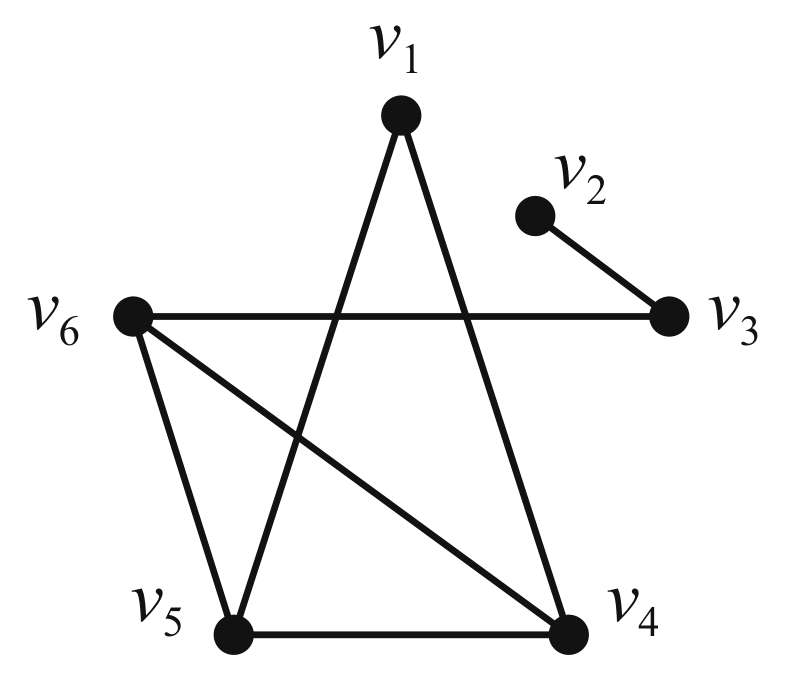
\includegraphics[height=3.2cm]{figure_1_29.png}
\end{column}
\begin{column}{0.54\textwidth}
\large
\[
A=\begin{pmatrix}
0&0&0&1&1&0\\
0&0&1&0&0&0\\
0&1&0&0&0&1\\
1&0&0&0&1&1\\
1&0&0&1&0&1\\
0&0&1&1&1&0
\end{pmatrix}.
\]
\centering
{\small Rows and columns follow $v_1,\ldots,v_6$.}
\end{column}
\end{columns}
\vfill
{\tiny Source: Harris, Hirst, and Mossinghoff, \emph{Combinatorics and Graph Theory}, 2nd ed., p.~22, Figure 1.29 and its adjacency matrix.}
\end{frame}


\begin{frame}{Remarks}
\normalsize
\begin{enumerate}
  \setlength{\itemsep}{0.16cm}
  \item For simple graphs (no loops or self-edges), every entry on the main diagonal is $0$.
  \item Adjacency matrices of undirected graphs are symmetric: $A=A^{\mathsf T}$.
  \item Different orderings of the vertices can produce different adjacency matrices.
\end{enumerate}

\vspace{0.18cm}
\begin{block}{Fact}
If $A$ and $B$ are adjacency matrices for the same graph $G$, there is a permutation of the vertices such that applying it to both the rows and the columns of $A$ gives $B$.
\end{block}

\vspace{0.12cm}
\begin{block}{Fact}
If graphs $G_1$ and $G_2$ have adjacency matrices $A_1$ and $A_2$, and applying the same permutation to the rows and columns of $A_1$ gives $A_2$, then $G_1$ and $G_2$ are isomorphic.
\end{block}
\end{frame}


\begin{frame}{Squares of Adjacency Matrices}
\normalsize
\textbf{Remark.} What does $A^2$ tell us about our graph?

\vspace{0.10cm}
\begin{columns}[c,onlytextwidth]
\begin{column}{0.43\textwidth}
\centering
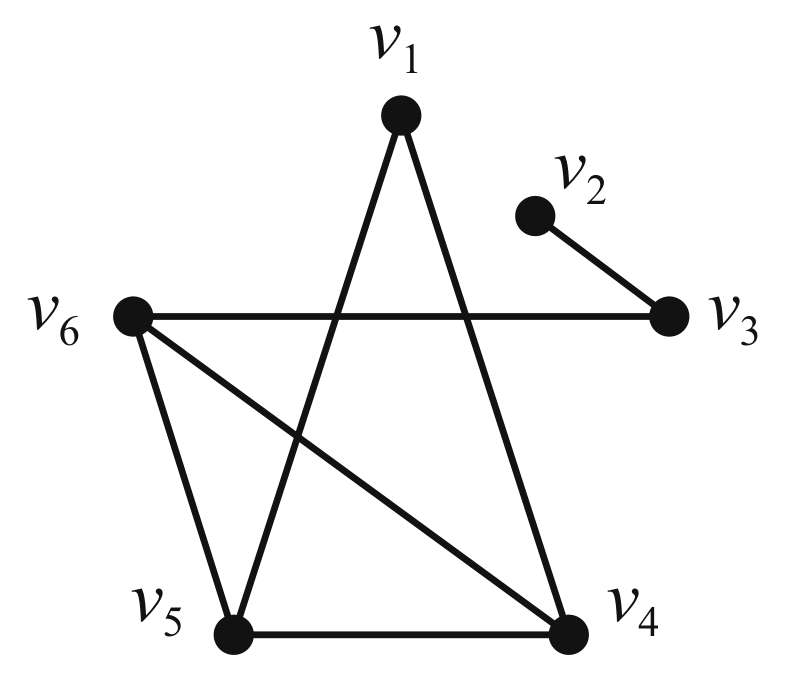
\includegraphics[height=2.65cm]{figure_1_29.png}
\end{column}
\begin{column}{0.54\textwidth}
\[
A=\begin{pmatrix}
0&0&0&1&1&0\\
0&0&1&0&0&0\\
0&1&0&0&0&1\\
1&0&0&0&1&1\\
1&0&0&1&0&1\\
0&0&1&1&1&0
\end{pmatrix}.
\]
\end{column}
\end{columns}
\vspace{-0.10cm}
\[
\begin{aligned}
[A^2]_{1,6}
 &= (0,0,0,1,1,0)\cdot(0,0,1,1,1,0)\\
 &= (0\cdot0)+(0\cdot0)+(0\cdot1)+(1\cdot1)+(1\cdot1)+(0\cdot0)\\
 &= 2.
\end{aligned}
\]
\vspace{-0.20cm}
\begin{block}{Notice}
Each non-zero term in the above sum corresponds to a walk of length $2$ from $v_1$ to $v_6$. Hence, $[A^2]_{1,6}$ counts the number of two-edge walks from $v_1$ to $v_6$.
\end{block}
\vfill
{\tiny Source: Harris, Hirst, and Mossinghoff, \emph{Combinatorics and Graph Theory}, 2nd ed., pp.~22--23, Figure 1.29.}
\end{frame}


\begin{frame}[t]{Theorem}
\begin{block}{Theorem 1.7}
For a graph $G$ with ordered vertices $v_1,\ldots,v_n$ and adjacency matrix $A$, the entry $[A^k]_{i,j}$ counts the walks of length $k$ from $v_i$ to $v_j$, for every integer $k\geq 1$.
\end{block}
\vfill
\end{frame}

\begin{frame}[t]{Proof of Theorem}
\begin{block}{Theorem 1.7}
For a graph $G$ with ordered vertices $v_1,\ldots,v_n$ and adjacency matrix $A$, the entry $[A^k]_{i,j}$ counts the walks of length $k$ from $v_i$ to $v_j$, for every integer $k\geq 1$.
\end{block}

\begin{block}{Proof}
\footnotesize
Induct on $k$. For $k=1$, the assertion is precisely the definition of $A$.

\smallskip
Assume the assertion holds for $k-1$. A walk of length $k$ from $v_i$ to $v_j$ has a unique penultimate vertex $v_h\in N(v_j)$. Removing its final edge leaves a walk of length $k-1$ from $v_i$ to $v_h$; conversely, every such walk can be extended by the edge $v_hv_j$.

\smallskip
By the induction hypothesis, the number of length-$k$ walks is therefore
\[
\sum_{v_h\in N(v_j)}[A^{k-1}]_{i,h}
=\sum_{h=1}^{n}[A^{k-1}]_{i,h}[A]_{h,j}
=[A^k]_{i,j}.
\]
This completes the induction.\hfill$\square$
\end{block}
\vfill
\end{frame}


\begin{frame}[t]{Corollary}
\begin{block}{Corollary 1.8}
Let $A$ be the adjacency matrix of $G$, with vertices ordered as $v_1,\ldots,v_n$. If $d(v_i,v_j)=x$, then
\[
[A^k]_{i,j}=0 \qquad\text{for every integer }1\leq k<x.
\]
\end{block}

\vspace{0.45cm}
\textbf{Question.} What is the proof?

\vfill
\end{frame}


\begin{frame}[t]{Theorem}
\begin{block}{Definition}
For a graph $G$ of order $n$ with adjacency matrix $A$, and an integer $k\geq 1$, define
\[
S_k=I+A+A^2+\cdots+A^k,
\]
where $I$ is the $n\times n$ identity matrix.
\end{block}

\smallskip
\textbf{Remark.} All entries are nonnegative integers, so
$[S_k]_{i,j}\leq [S_{k+1}]_{i,j}$ for every $i,j$.

\begin{block}{Theorem 1.9}
\small
Suppose $G$ is connected and has vertices $v_1,\ldots,v_n$, with $n\geq 2$.
\begin{enumerate}
\setlength{\itemsep}{0.15cm}
\item $\operatorname{ecc}(v_j)$ is the least positive $k$ for which row $j$ of $S_k$ has no zero entries.
\item $\operatorname{rad}(G)$ is the least positive $r$ for which some row of $S_r$ has only positive entries.
\item $\operatorname{diam}(G)$ is the least positive $m$ for which every entry of $S_m$ is positive.
\end{enumerate}
\end{block}
\end{frame}


\begin{frame}[t]{Proof of Theorem}
\begin{block}{Theorem 1.9: Part 1}
For a connected graph $G$ with at least two vertices, if $k$ is the least positive integer for which row $j$ of $S_k$ has no zero entries, then
\[
\operatorname{ecc}(v_j)=k.
\]
\end{block}

\smallskip
\textbf{Remark.} Parts 2 and 3 are left as exercises.

\begin{block}{Proof}
\small
Because every entry in row $j$ of $S_k$ is positive, every vertex can be reached from $v_j$ by a walk of length at most $k$. Thus
$\operatorname{ecc}(v_j)\leq k$.

\smallskip
If $k=1$, then $\operatorname{ecc}(v_j)=1$, since $G$ has at least two vertices.

\smallskip
If $k>1$, minimality of $k$ means that row $j$ of $S_{k-1}$ contains a zero. The corresponding vertex is at distance greater than $k-1$ from $v_j$, so $\operatorname{ecc}(v_j)\geq k$.

\smallskip
Consequently, $\operatorname{ecc}(v_j)=k$.\hfill$\square$
\end{block}
\end{frame}


\begin{frame}[t]{Creating a New Matrix, $M$}
\begin{block}{Construction}
\small
Let $G$ be a connected graph with vertices $v_1,\ldots,v_n$ and adjacency matrix $A$. Recall that
\[
S_k=I+A+A^2+\cdots+A^k.
\]
Define an $n\times n$ matrix $M$ as follows:
\begin{enumerate}
\setlength{\itemsep}{0.25cm}
\item Set $[M]_{i,i}=0$ for every $i$.
\item For $i\neq j$, let $[M]_{i,j}$ be the least positive integer $k$ such that $[S_k]_{i,j}\neq 0$.
\end{enumerate}
\end{block}

\vspace{0.05cm}
\begin{block}{Remark}
By construction, each entry records the corresponding distance:
\[
[M]_{i,j}=d(v_i,v_j).
\]
The matrix $M$ is called the \textbf{distance matrix} of $G$.
\end{block}
\end{frame}


\begin{frame}[t]{Graph Model: The Acquaintance Graph}
\begin{block}{The Acquaintance Graph}
Each vertex represents a person. Two vertices are joined by an edge when the corresponding people know each other.
\end{block}
\small
\begin{itemize}
\setlength{\itemsep}{0.10cm}
\item We may model a classroom, a neighbourhood, or the world's population.
\item A path is a chain of acquaintances; distance counts the fewest links needed.
\item The ``six degrees of separation'' claim translates to $\operatorname{diam}(G)\leq 6$ for the worldwide graph. It is difficult to verify: the graph is huge and changes over time.
\end{itemize}

\vspace{0.05cm}
\centering
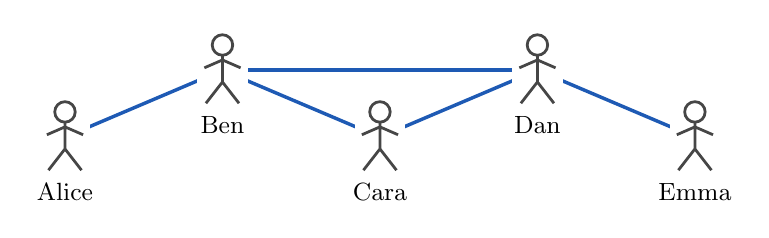
\begin{tikzpicture}[x=1cm,y=1cm]
\coordinate (Alice) at (0,0);
\coordinate (Ben) at (2,0.85);
\coordinate (Cara) at (4,0);
\coordinate (Dan) at (6,0.85);
\coordinate (Emma) at (8,0);
\foreach \a/\b in {Alice/Ben,Ben/Cara,Cara/Dan,Dan/Emma,Ben/Dan}
  \draw[edge] (\a) -- (\b);
\foreach \name in {Alice,Ben,Cara,Dan,Emma}{
  \begin{scope}[shift={(\name)}]
    \fill[white] (-0.32,-0.47) rectangle (0.32,0.54);
    \draw[DarkGray,line width=1pt] (0,0.32) circle (0.13);
    \draw[DarkGray,line width=1pt] (0,0.19)--(0,-0.15)
      (-0.23,0.03)--(0,0.13)--(0.23,0.03)
      (-0.21,-0.42)--(0,-0.15)--(0.21,-0.42);
    \node[below,font=\small] at (0,-0.46) {\name};
  \end{scope}
}
\end{tikzpicture}
\par\smallskip
{\footnotesize An illustrative acquaintance graph: each edge means ``knows.''}
\end{frame}


\begin{frame}[t]{Graph Model: The Hollywood Graph}
\begin{block}{The Hollywood Graph}
Vertices represent actors. Two actors are joined by an edge if they have appeared in a movie together.
\end{block}

\vspace{0.18cm}
\begin{columns}[c,onlytextwidth]
\begin{column}{0.49\textwidth}
\small
An actor's \textbf{Bacon number} is their graph distance from Kevin Bacon: the fewest shared-movie links needed to reach him.

\medskip
Bacon has number $0$; his co-stars have number $1$. An actor with no connection to him has number $\infty$.

\medskip
The \textbf{Kevin Bacon Game} challenges people to find short chains connecting actors to him---a playful example of ``six degrees of separation.''

\medskip
Being drawn in the middle does not by itself make Bacon a graph-theoretic center!
\end{column}
\begin{column}{0.48\textwidth}
\centering

\begin{tikzpicture}[scale=0.94]
\foreach \i in {0,...,11}{
  \coordinate (a\i) at ({30*\i}:1.6);
  \draw[edge] (0,0)--(a\i);
}
\foreach \i/\ang/\near in {0/15/0,1/105/3,2/195/6,3/285/9}{
  \coordinate (b\i) at (\ang:2.3);
  \draw[edge] (b\i)--(a\near);
  \fill[DarkGray] (b\i) circle (2.7pt);
}
\foreach \i/\j in {0/1,2/3,3/4,5/6,7/8,9/10,10/11}
  \draw[edge] (a\i)--(a\j);
\foreach \i in {0,...,11}
  \fill[DarkGray] (a\i) circle (2.7pt);
\fill[white] (0,0) ellipse (0.68 and 0.8);
\draw[RamRed,line width=1.3pt] (0,0.39) circle (0.17);
\draw[RamRed,line width=1.3pt] (0,0.22)--(0,-0.21)
  (-0.29,0.01)--(0,0.15)--(0.29,0.01)
  (-0.26,-0.56)--(0,-0.21)--(0.26,-0.56);
\node[below,fill=white,inner sep=2pt,font=\footnotesize\bfseries] at (0,-0.57) {Kevin Bacon};
\end{tikzpicture}
\par\smallskip
{\scriptsize Schematic only; dots represent other actors.}
\end{column}
\end{columns}
\end{frame}

\begin{frame}[t]{Graph Model: Mathematical Collaboration Graph}
\begin{block}{The Mathematical Collaboration Graph}
Vertices represent researchers. Two researchers are joined by an edge if they have coauthored a paper.
\end{block}

\vspace{0.18cm}
\begin{columns}[c,onlytextwidth]
\begin{column}{0.49\textwidth}
\small
A researcher's \textbf{Erd\H{o}s number} is their graph distance from Paul Erd\H{o}s: the fewest coauthorship links needed to reach him.

\medskip
Erd\H{o}s has number $0$, and his coauthors have number $1$. Coauthors of those researchers have number $2$, unless a shorter connection exists.

\medskip
Erd\H{o}s had hundreds of collaborators. His number system highlights connections across mathematics.

\medskip
A researcher outside his connected component has Erd\H{o}s number $\infty$.
\end{column}
\begin{column}{0.48\textwidth}
\centering

\begin{tikzpicture}[scale=0.94]
\foreach \i in {0,...,11}{
  \coordinate (a\i) at ({30*\i}:1.6);
  \draw[edge] (0,0)--(a\i);
}
\foreach \i/\ang/\near in {0/15/0,1/105/3,2/195/6,3/285/9}{
  \coordinate (b\i) at (\ang:2.3);
  \draw[edge] (b\i)--(a\near);
  \fill[DarkGray] (b\i) circle (2.7pt);
}
\foreach \i/\j in {0/1,2/3,3/4,5/6,7/8,9/10,10/11}
  \draw[edge] (a\i)--(a\j);
\foreach \i in {0,...,11}
  \fill[DarkGray] (a\i) circle (2.7pt);
\fill[white] (0,0) ellipse (0.68 and 0.8);
\draw[RamRed,line width=1.3pt] (0,0.39) circle (0.17);
\draw[RamRed,line width=1.3pt] (0,0.22)--(0,-0.21)
  (-0.29,0.01)--(0,0.15)--(0.29,0.01)
  (-0.26,-0.56)--(0,-0.21)--(0.26,-0.56);
\node[below,fill=white,inner sep=2pt,font=\footnotesize\bfseries] at (0,-0.57) {Paul Erd\H{o}s};
\end{tikzpicture}
\par\smallskip
{\scriptsize Schematic only; dots represent other researchers.}
\end{column}
\end{columns}
\end{frame}


\begin{frame}[t]{Small World Networks}
The acquaintance graph captures the feeling that people are connected through surprisingly short chains. But the full network is enormous and constantly changing, so smaller graph models are easier to study.

\medskip
To reflect this phenomenon, a small world network should have several properties:

\begin{block}{1. Many mutual acquaintances}
People should often have shared neighbours. Complete graphs have plenty of these, but they are unrealistic: not everyone knows everyone else.
\end{block}

\medskip
\begin{block}{2. Relatively few edges}
The graph should be \textbf{sparse}: only a small fraction of all possible pairs should be adjacent. Each person knows only a small part of the population.
\end{block}
\end{frame}

\begin{frame}[t]{Small World Networks continued...}
\begin{block}{3. Short distances}
\small\setlength{\abovedisplayskip}{5pt}\setlength{\belowdisplayskip}{5pt}
The \textbf{characteristic path length} $L_G$ is the average distance over all distinct vertex pairs. For a connected graph with $n\geq 2$ vertices,
\[
L_G=\frac{2}{n(n-1)}\sum_{1\leq i<j\leq n}d(v_i,v_j).
\]
It is also the mean of the off-diagonal entries of the distance matrix.
\end{block}

\begin{block}{4. Substantial clustering}
\small\setlength{\abovedisplayskip}{5pt}\setlength{\belowdisplayskip}{5pt}
Local groups should contain a high proportion of edges.

\smallskip
The book measures clustering within the closed neighbourhood $N[v]$:
\[
\operatorname{cc}(v)=\frac{|E(G[N[v]])|}{\binom{1+\deg(v)}{2}},
\qquad
\operatorname{CC}(G)=\frac{1}{n}\sum_{v\in V(G)}\operatorname{cc}(v).
\]
Thus $\operatorname{cc}(v)$ is the fraction of possible edges present in $G[N[v]]$.
\end{block}

\end{frame}


\begin{frame}[t]{Interesting Note}
\begin{block}{Erd\H{o}s has a Bacon number!}
If shared appearances in documentaries count, Paul Erd\H{o}s has a \textbf{Bacon number of $3$}, as reported in the textbook.

\medskip
Erd\H{o}s is the subject of the 1993 documentary \emph{N is a Number}. Alec Guinness appears briefly in the film and has Bacon number $2$, providing a link from Erd\H{o}s to Kevin Bacon.
\end{block}

\vspace{0.25cm}
\begin{block}{Does Bacon have an Erd\H{o}s number?}
The textbook reports no known chain of coauthored research papers connecting Kevin Bacon to Erd\H{o}s. On that account, Bacon's Erd\H{o}s number is $\infty$.

\medskip
A shared film appearance creates an edge in the Hollywood graph; a joint research paper creates an edge in the mathematical collaboration graph.
\end{block}
\end{frame}


\begin{frame}{Next time}
\centering
\vfill
{\Huge\color{RamBlue} Trees}
\vfill
\end{frame}

\end{document}
